\newpage
\subsection{Diagrammi UML comportamentali}
In questa sezione sono riportati alcuni diagrammi comportamentali a corredo dei diagrammi dei casi d'uso e UML delle classi che illustrano il funzionamento della prima versione dell'applicazione.

I diagrammi UML riportati di seguito sono altamente descrittivi, in modo da essere utilizzabili per mostrare all'utente in maniera intuitiva il funzionamento dell'applicazione, pur rispettando le direttive UML.\bigskip

\textbf{Diagramma di sequenza: Accesso Configuratore}\newline
In Figura \ref{fig:Sequence diagram 1.1} è riportato il diagramma di sequenza che rappresenta gli step che caratterizzano l'interazione dell'utente con l'applicazione per consentire all'utente Configuratore di accedere all'applicazione.\newline Si presenta di seguito la descrizione ad alto livello delle azioni che si verificano in corrispondenza di ogni numero riportato sulle frecce:

\begin{enumerate}
    \item L'utente richiede di accedere al proprio profilo
    \item L'applicazione richiede all'utente di inserire il proprio username nell'interfaccia presentatagli
    \item L'utente inserisce il proprio username
    \item L'interfaccia comunica al Controller dell'applicazione lo username inserito dall'utente
    \item Il Controller verifica l'esistenza dello username all'interno dell'elenco degli utenti
    \item Se lo username esiste all'interno dell'elenco degli utenti il Controller manda un messaggio di conferma della correttezza dei dati inseriti all'interfaccia
    \item L'interfaccia dell'applicazione richiede all'utente la password
    \item L'utente inserisce la propria password
    \item L'interfaccia comunica al Controller dell'applicazione la password inserita dall'utente
    \item Il Controller verifica la correttezza della password
    \item Se la password è corretta il Controller comunica all'interfaccia che il login è stato effettuato correttamente
    \item L'interfaccia comunica all'utente che il login è stato effettuato correttamente
    \item Se la password è errata il Controller comunica all'interfaccia che il login è fallito
    \item L'interfaccia comunica all'utente che il login è fallito
    \item Se lo username è inesistente il Controller comunica all'interfaccia che il login è fallito
    \item L'interfaccia comunica all'utente che il login è fallito
\end{enumerate}

\begin{figure}[!]
\centering
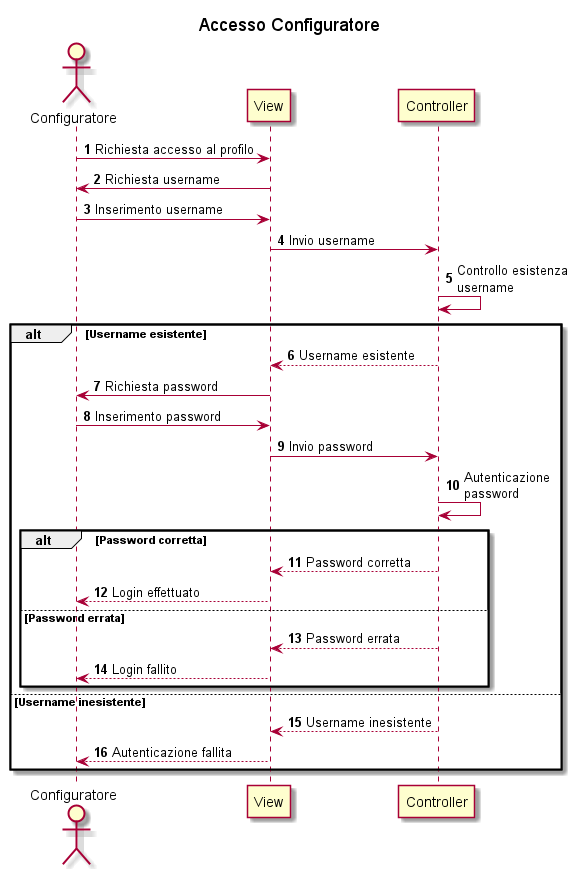
\includegraphics[width=0.6\textwidth]{imagesV1/Sequence diagram-Accesso configuratore.png}
\caption{\label{fig:Sequence diagram 1.1}Diagramma di sequenza: Accesso configuratore - Versione 1}
\end{figure}\bigskip

\newpage
\textbf{Diagramma degli Stati: Ciclo di vita dell'utente Configuratore}\newline
In Figura \ref{fig:State diagram 1.1} è rappresentato il ciclo di vita dell'utente Configuratore: a seconda dell'azione che esso intraprende nei confronti dell'applicazione il Configuratore si trova in un determinato stato.\newline L'accesso all'applicazione può avvenire o in qualità di primo accesso oppure come accesso ordinario: nel caso si tratti di un primo accesso il configuratore si riconduce allo stato "CreazioneProfilo" in cui avviene la creazione di un nuovo profilo Configuratore a cui segue un necessario cambio delle credenziali, mentre nel caso si tratti di un login ordinario l'utente accede direttamente al menu principale. \newline 
In tutti i passaggi di stato si considera la situazione ideale in cui non vi siano errori nell'esecuzione delle operazioni. Nel caso in cui si verifichino errori di esecuzione allora è lasciato sottinteso il passaggio attraverso uno stato di Errore prima di tornare al menu principale.

\begin{figure}[b!]
\centering
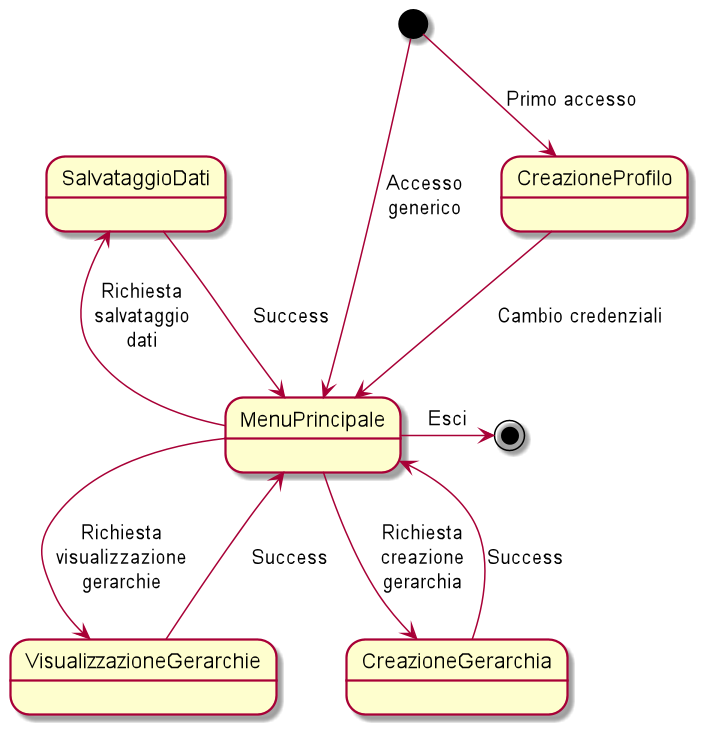
\includegraphics[width=0.7\textwidth]{imagesV1/State diagram - Ciclo di vita del configuratore.png}
\caption{\label{fig:State diagram 1.1}Ciclo di vita del Configuratore - Versione 1}
\end{figure}\bigskip